\documentclass{standalone}
\usepackage{tikz}
\usepackage{sansmath}
\usepackage{helvet}

\begin{document}
\sansmath
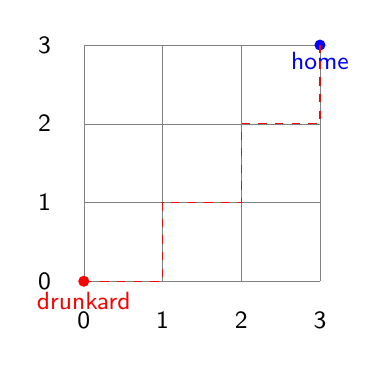
\begin{tikzpicture}
    % Use sans-serif font and smaller font size
    \tikzstyle{every node}=[font=\sffamily\small]

    % Draw the grid
    \draw[step=1cm,gray,very thin] (0,0) grid (3,3);

    % Label the axes
    \foreach \x in {0,1,2,3} \node at (\x,-0.5) {\x};
    \foreach \y in {0,1,2,3} \node at (-0.5,\y) {\y};

    % Draw the points
    \fill[red] (0,0) circle (2pt);
    \fill[blue] (3,3) circle (2pt);

    % Label the points below the dots
    \node[red] at (0,-0.25) {drunkard};
    \node[blue] at (3,2.8) {home};

    % Draw the dashed line path from (0,0) to (3,3)
    \draw[red, dashed] (0,0) -- (1,0) -- (1,1) -- (2,1) -- (2,2) -- (3,2) -- (3,3);
    
\end{tikzpicture}
\end{document}